%!TEX root = thesis.tex

\chapter{Follow-Up User Study}
\label{chap:follow-up-user-study}

A follow-up user study was conducted to evaluate the set of refined visualisations and to address some of the limitations identified in the first user study. This included providing a valid baseline for the study (the \emph{no visualisation} condition) and reducing the visualisations to more meaningful representations.

% The previous visualisation prototype and user study also lacked a clear baseline.  with an analysis and comparison to a live coded performance without -previous study did not have a baseline - this was to be remedied

It was hypothesised that the visualisation prototype would result in higher understanding at the end of the performance and that enjoyment would remain steady throughout both performances.

\section{Method}

Two independent audiences ($N=14+11=25$) were recruited through on campus advertisement (see Appendix~\ref{appendix:follow-up-user-study-advertisement}). Each group was exposed to two live coding musical performances. One of the performances displayed only the source code of the performance while the other displayed the source code with the refined visualisation prototype as an underlay (see Chapter~\ref{chap:visualisation-refinement}).

The first group was subjected to the \emph{visualisation} condition, followed by the \emph{no visualisation} condition. The conditions were swapped for the second group, with the audience exposed to the \emph{no visualisation} condition first followed by the \emph{visualisation} condition.

Again, over the course of these performances, each audience member completed a survey consisting of four sections: demographic information, their opinion of the first piece, their opinion of the second piece and questions about the performance overall. 

Two additional questions were asked to get an impression of the audience's understanding at specific stages of the performance:

\begin{itemize}
\item What do you think the performer was doing in the very early stages of the performance? \qlab{question:study-3-early-stages}
\item What do you think the performer was doing in the very last stages of the performance? \qlab{question:study-3-last-stages}
\end{itemize}


% Table showing the criteria for understanding
% \begin{table}
% \begin{center}
% \begin{tabular}{ |l|p{7cm}| }
% \hline
% Understanding Level & Concepts \\ \hline
% \multirow{3}{*}{Basic} & Identify functions or note distinctions between functions \\
%  & Identify that the programmer has started writing a function \\
%  & Refer to text selection or text editing \\ \hline
% \multirow{3}{*}{Intermediate} & Identify when the programmer begins editing or modifying a function \\
%  & Identify the activation of a function\\
%  & Identify the deactivation of a function \\ \hline
% \multirow{3}{*}{Advanced} & Identify when an error occurs \\
%  & Identify function mapping to instruments or sound output \\
%  & Identify programmer long-term goals \\
% \hline
% \end{tabular}
% \end{center}
% \caption[Understanding levels]{Levels for evaluating audience understanding.}
% \label{table:understanding-levels}
% \end{table}



\section{Participants}

Of the 25 total participants over the two performances $12\%$ were female. $64\%$ of the audience had not been to a live coding performance before and $80\%$ had not attended the previous live coding user study. The background of the audience included $56\%$ that listened to music regularly, $28\%$ that played an instrument and $72\%$ who programmed for their hobby, job or study.

\section{Results}

\begin{figure}
  \centering
  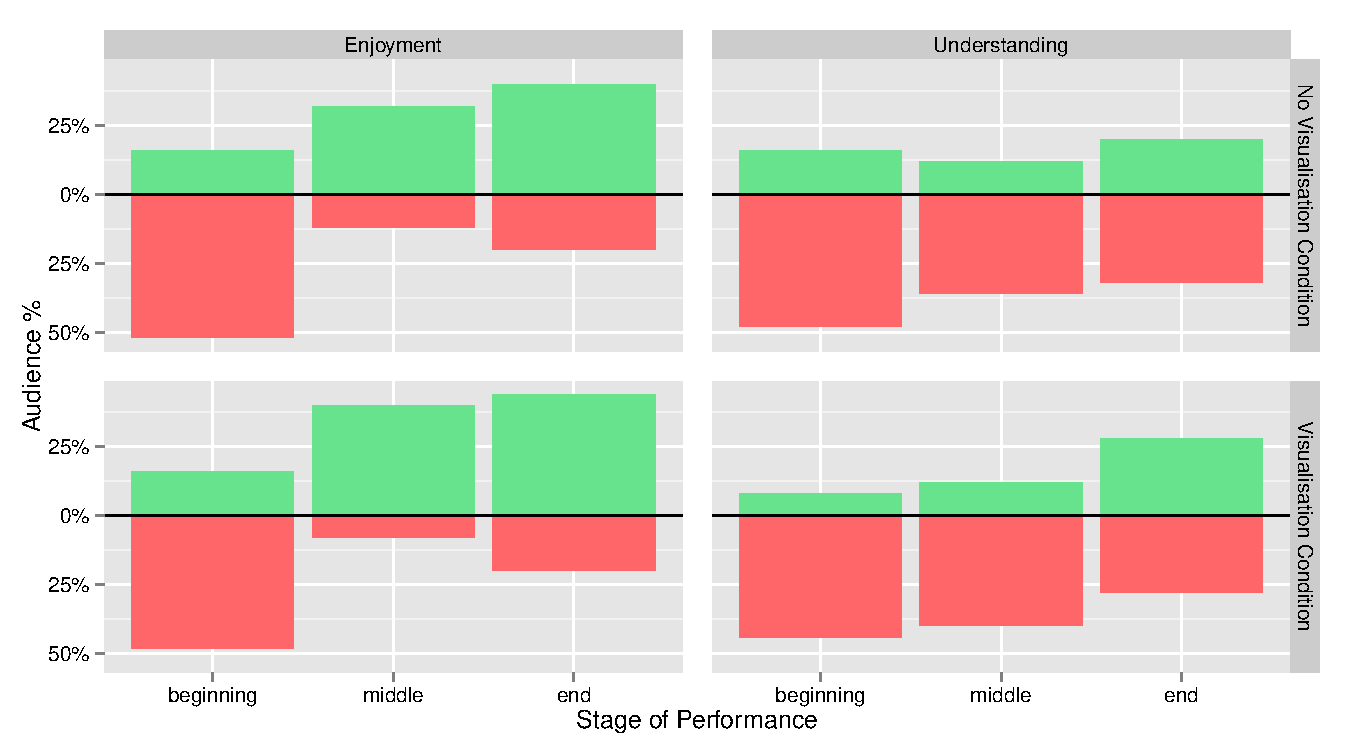
\includegraphics[width=\columnwidth]{../study-3/results/dimension-condition-study-3.pdf}
  \caption[Follow-up user study survey condition and dimension results]{Percentage of the audience reporting ``high'' (green - above the line) and ``low'' (red - below the line) enjoyment and understanding over the beginning, middle and end stages of the performances for the no visualisation and visualisation conditions. The remaining population, not shown here, reported ``medium'' levels of enjoyment or understanding.}
  \label{fig:dimension-condition-follow-up-user-study}
\end{figure}

The audience-reported enjoyment and understanding responses from the survey were evaluated for the two conditions as described below. A summary of the results can be seen in Figure~\ref{fig:dimension-condition-follow-up-user-study}.

\subsection{Enjoyment}

\begin{figure}
\centering
\begin{subfigure}{\textwidth}
  \centering
  \includegraphics[width=\columnwidth,page=7]{../images/graphs/condition-dimension.pdf}
  \caption[No visualisation condition enjoyment detailed survey results]{Audience reported enjoyment level for the \textbf{no visualisation} condition.}
  \label{fig:no-visualisation-enjoyment}
\end{subfigure}\\
\vspace{15mm}
\begin{subfigure}{\textwidth}
  \centering
  \includegraphics[width=\columnwidth,page=8]{../images/graphs/condition-dimension.pdf}
  \caption[Visualisation condition enjoyment detailed survey results]{Audience-reported enjoyment level for the \textbf{visualisation} condition.}
  \label{fig:visualisation-enjoyment}
\end{subfigure}
\vspace{15mm}
\caption[Follow-up user study enjoyment survey responses]{Audience reported enjoyment during the beginning, middle and end of the performance for the no visualisation and visualisation conditions. Line width at each stage indicates proportion of the audience reporting high, medium or low enjoyment, and line colour connecting each section of the performance is determined by the enjoyment level at the \emph{beginning} of the performance.}
\label{fig:follow-up-user-study-condition-enjoyment}
\end{figure}

Audiences were asked to state if they thought the source code projection helped their enjoyment of the performance and if they thought the visualisations helped their enjoyment of the performance. Of the audience, $60\%$ stated that projection of the source code helped their enjoyment of the performance directly while $16\%$ stated that the visualisations helped their enjoyment directly.

Levels of enjoyment throughout the performance were surveyed for the \emph{beginning}, \emph{middle} and the \emph{end} phases of the performance. A comparison of the enjoyment between the no visualisation condition and the visualisation condition is available in Figure~\ref{fig:no-visualisation-enjoyment} and Figure~\ref{fig:visualisation-enjoyment}.

Final levels of enjoyment between the two conditions differed only slightly. With no visualisation, $20\%$ stated that they had low enjoyment, $40\%$ stated that they had medium enjoyment and $40\%$ stated that they had high enjoyment. With visualisations, $20\%$ stated low enjoyment, $36\%$ stated medium enjoyment and $44\%$ stated high enjoyment.

\subsection{Understanding}

\begin{figure}
\centering
\begin{subfigure}{\textwidth}
  \centering
  \includegraphics[width=\columnwidth,page=5]{../images/graphs/condition-dimension.pdf}
  \caption[No visualisation condition understanding detailed survey results]{Audience reported understanding level for the \textbf{no visualisation} condition.}
  \label{fig:no-visualisation-understanding}
\end{subfigure}\\
\vspace{15mm}
\begin{subfigure}{\textwidth}
  \centering
  \includegraphics[width=\columnwidth,page=6]{../images/graphs/condition-dimension.pdf}
  \caption[Visualisation condition understanding detailed survey results]{Audience-reported understanding level for the \textbf{visualisation} condition.}
  \label{fig:visualisation-understanding}
\end{subfigure}
\vspace{15mm}
\caption[Follow-up user study understanding survey responses]{Audience reported understanding during the beginning, middle and end of the performance for the no visualisation and visualisation conditions. Line width at each stage indicates proportion of the audience reporting high, medium or low understanding, and line colour connecting each section of the performance is determined by the understanding level at the \emph{beginning} of the performance.}
\label{fig:follow-up-user-study-condition-understanding}
\end{figure}

Audiences were asked to state if they thought the source code projection helped their understanding of the performance and if they thought the visualisations helped their understanding of the performance. Of the audience, $76\%$ stated that projection of the code helped their understanding of the performance directly while $32\%$ stated that the visualisations helped their understanding directly.

Levels of understanding throughout the performance were surveyed for the \emph{beginning}, \emph{middle} and the \emph{end} phases of the performance. A comparison of the understanding between the no visualisation condition and the visualisation condition is available in Figure~\ref{fig:no-visualisation-understanding} and Figure~\ref{fig:visualisation-understanding}.

Levels of understanding also differed slightly between the two conditions. With no visualisation, $32\%$ stated that they had low understanding, $48\%$ stated that they had medium understanding and $20\%$ stated that they had high understanding. With visualisations, $28\%$ stated low understanding, $44\%$ stated medium understanding and $28\%$ stated high understanding.

%%%%%%%%%%%%%%%%%%%%%%%%%%%%%%%%%%%%%%%%%%%%%%%%%%%%%%%%%%%%%%%%%%%%%%%%%%%%%%%%%
After each performance, two additional questions were asked (see Questions~\ref{question:study-3-early-stages} and \ref{question:study-3-last-stages}). Results of these questions... \more
% Results from these questions were evaluated against a criteria for understanding level (see Table~\ref{table:understanding-levels}).
%%%%%%%%%%%%%%%%%%%%%%%%%%%%%%%%%%%%%%%%%%%%%%%%%%%%%%%%%%%%%%%%%%%%%%%%%%%%%%%%%

\subsection{Liveness}

After exposing the audience to both conditions, the audience was asked if the projected source code or visualisations helped to communicate the feeling that the performances were live. Of the twenty-five responses, eighteen indicated that the projection of the source code helped, though the audience overall was experienced in programming. 

Results of this question reflected the audience opinion of the visualisations. Some responses indicated that: ``Yes. Live code editing [helped to communicate the liveness], but visualisations showed what coder was looking at and editing as well as what was running.''. In contrast, members of the audience stated that the ``visualisations [were] not really useful, didn't seem in sync with the music and [had] no obvious meaning''. However, most of the audience ($64\%$) focussed on the source code or musical aspects of the performance in their discussion of liveness.

\section{Discussion}

Overall, only minor differences were observed between the no visualisation and visualisation conditions. Mirroring the previous user study, a pattern of lower understanding was seen with the visualisations during the beginning of the performance. 

\more

% This 

% Content Analysis Questions:
% Which data are analysed?
% How are they defined?
% What is the population from which they are drawn?
% What is the context relative to which the data are analysed?
% What are the boundaries of the analysis?
% What is the target of the inferences?



\subsection{Comparison to Previous Study}

\more

% From presentation (for Figure~\ref{fig:enjoyment-final}):

% [results of this study and the results of previous user study gave rise to the following….]
% this graph shows the percent of the audience reporting their levels of enjoyment over the three stages of the performance for the two conditions of “no visualisation” and “with visualisation” 
% the no visualisation condition is marked as a solid line
% the visualisation condition is marked as a dotted line
% the percent of the audience reporting high is marked in green, reporting medium is marked in blue and reporting low is marked in red
% a smaller percentage of the low group and a larger percentage of the high group would be desirable

% - for example, during the beginning of the performance, for the visualisation condition, 30% of the audience stated that they had low enjoyment while for the no visualisation, 50% of the audience stated that they had low enjoyment

% this graph shows an overall increase in enjoyment consistently throughout the performance
% increase in a high level of enjoyment with the visualisation, particularly during the middle of the performance
% in summary, these results indicate that there is a clear shift upwards in enjoyment throughout the performance, with the visualisations always performing equal or better than the no visualisation condition

% % From presentation (for Figure~\ref{fig:understanding-final}):

% this graph is for understanding and is a similar format to the previous
% coloured lines show percent of audience with that level of understanding

% shows an increase in the percent reporting medium understanding with the visualisation compared to without… 
% visualisations appears to help audiences reporting low understanding
% however, little impact on the percent reporting high levels of understanding
% -  in summary, it shows a consistent increase throughout the performance for all except those with high understanding


\subsection{Limitations}

A number of factors were identified that could influence the validity of the user study results.

The visualisations suffered from being obscured by the source code displayed on the projection screen. However, compared to the initial user study, the visualisations were logically placed in relation to the source code, from top to bottom, in the order the functions appeared in the code to attempt to counteract this interference.

Nevertheless, one member of the audience stated that ``the visualisation made sense of the separate parts [of the code] so you could track each easier but [the visualisations] were difficult to see''. The difficulty in seeing the visualisations was discussed by a number of members of the audience, generally stating that the visualisations were projected too faintly behind the source code.

% Due to a technical oversight during the first performance, the visualisation underlay was difficult to distinguish. 
% This was this was intentionally left the same for the second performance group.

A large proportion of the audience stated that they had coding experience. This may have influenced the preference for seeing the source code during live coding performances. An audience experienced in coding may be less interested in viewing visualisations and have a preference for viewing code directly without anything interferring with the source code.

The small sample size demonstrated only small differences between the two conditions examined. A larger sample may have provided more significance in the results. \more

Finally, as with the first user study, musical and visual preference may have contributed to the results of the survey. Again, an attempt was made to mitigate this through similar musical styles through all performances.

\section{Summary}

This study identifies some small differences between live coding with and without visualisations. A larger proportion of the audience had high enjoyment during the middle of the performance when a visualisation was displayed than without. Similarly, the visualisations resulted in a small increase in the proportion of the audience reporting high understanding. However, this was offset by fewer reporting high understanding at the beginning of the performance. 

Although some variation was found, the sample size... \more









